\subsection{凸函数的连续性与可导性}

命题 5. 为使实值有限函数 f 在区间 I 上是凸的（相应地，严格凸的），必须且只需：对一切 \(a \in I\)，梯度

\[
p (\mathbf {M} _ {a} \mathbf {M} _ {x}) = \frac {f (x) - f (a)}{x - a}
\]

在 I ∩ ∁\{a\} 上是 x 的递增（相应地，严格递增）函数。

本命题是定义 1 和定义 2 以及 I, p.~23 中的引理的直接推论。

命题 6. 设 \(f\) 是区间 \(\mathbf{I} \subset \mathbf{R}\) 上的实值有限凸函数。那么，在每个内点 \(a\)（属于 \(\mathbf{I}\)）处，函数 \(f\) 连续，具有有限的右导数与左导数，并且 \(f_g'(a) \leqslant f_d'(a)\)。

事实上，对 \(x \in I\) 与 \(x > a\)，函数 \(x \mapsto \frac{f(x) - f(a)}{x - a}\) 递增（命题 5）且有下界，因为若 \(y < a\) 与 \(y \in I\)，就有

\[
\frac {f (y) - f (a)}{y - a} \leqslant \frac {f (x) - f (a)}{x - a}\tag{5}
\]

（依命题 5）；因此这个函数在点 \(a\) 处有有限的右极限；换言之，\(f_d'(a)\) 存在且有限；再者，在 (5) 中令 \(x\) 趋于 \(a\)（\(x > a\)），便得到

\[
\frac {f (y) - f (a)}{y - a} \leqslant f _ {d} ^ {\prime} (a)\tag{6}
\]

对一切属于 I 的 \(y < a\) 成立。同理可证 \(f_{g}^{\prime}(a)\) 存在，且

\[
f _ {d} ^ {\prime} (a) \leqslant \frac {f (x) - f (a)}{x - a}\tag{7}
\]

对 \(x \in I\) 以及 x \textgreater{} a 成立。在这最后一个不等式中令 x 趋于 \(a (x > a)\)，就得到 \(f_{g}^{\prime}(a) \leqslant f_{d}^{\prime}(a)\)。点 a 处左导数与右导数的存在性显然保证 f 在该点连续。

推论 1. 设 \(f\) 是 I 上的凸（相应地，严格凸）函数；若 \(a\) 与 \(b\) 是 I 的两个内点且 \(a < b\)，则有（图~3）

\pandocbounded{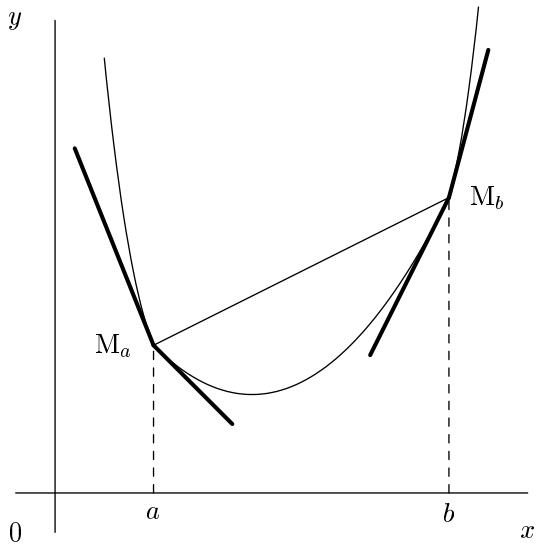
\includegraphics[keepaspectratio]{images/part001_a227d9e4.jpg}}\\
图 3

\[
f _ {d} ^ {\prime} (a) \leqslant \frac {f (b) - f (a)}{b - a} \leqslant f _ {g} ^ {\prime} (b)\tag{8}
\]

（相应地，

\[
f _ {d} ^ {\prime} (a) <   \frac {f (b) - f (a)}{b - a} <   f _ {g} ^ {\prime} (b)).\tag{9}
\]

二重不等式 (8) 由 (6) 与 (7) 经简单的记号改动而得。另一方面，若 \(f\) 严格凸，且 \(c\) 使得 \(a < c < b\)，则由 (8) 与命题 5 得

\[
f _ {d} ^ {\prime} (a) \leqslant \frac {f (c) - f (a)}{c - a} <   \frac {f (b) - f (a)}{b - a} <   \frac {f (b) - f (c)}{b - c} \leqslant f _ {g} ^ {\prime} (b)
\]

由此得 (9)。

推论 2. 若 f 在 I 上是凸的（相应地，严格凸的），则 \(f_{d}^{\prime}\) 与 \(f_{g}^{\prime}\) 在 I 的内部递增（相应地，严格递增）；I 中使 f 不可导的点所成的集是可数的，并且 \(f_{d}^{\prime}\) 与 \(f_{g}^{\prime}\) 在 f 可导的每一点处连续。

第一部分立即由 (8)（相应地，(9)）以及不等式

\[
f _ {g} ^ {\prime} (a) \leqslant f _ {d} ^ {\prime} (a).
\]

得出。另一方面，设 E 为 I 中使 f 不可导的内点 x 所成的集（即 \(f_{g}^{\prime}(x) < f_{d}^{\prime}(x)\)）。对每个 \(x \in E\)，设 \(J_{x}\) 为开区间 \(]f_{g}^{\prime}(x), f_{d}^{\prime}(x)[;\)；由 (8) 可知，若 x 与 y 是 E 中满足 x \textless{} y 的两点，则 u \textless{} v 对一切 \(u \in J_{x}\) 与一切 \(v \in J_{y}\) 成立；换言之，当 x 跑遍 E 时，非空开区间 \(J_{x}\) 两两不相交；这样的区间所成的集因此是可数的，从而 E 也是可数的。最后，\(f_{d}^{\prime}\)（相应地，\(f_{g}^{\prime}\)）递增，故它在 I 的每个内点 x 处都有右极限与左极限；于是 I, p.~18 的命题 6 表明，\(f_{d}^{\prime}\)（相应地，\(f_{g}^{\prime}\)）在点 x 处的右极限等于 \(f_{d}^{\prime}(x)\)，而其左极限等于 \(f_{g}^{\prime}(x)\)；由此即得推论的最后一部分。

设 \(f\) 是 \(I, a\) 上的凸函数，\(I\) 为其一个内点，\(D\) 为过点 \(M_a\) 的一条直线，其方程为 \(y - f(a) = \alpha(x - a)\)。由不等式 (8) 可知，若 \(f_g'(a) \leqslant \alpha \leqslant f_d'(a)\)，则图像 \(G\) 的每一点都位于 \(D\) 之上；并且若 \(f\) 严格凸，则 \(M_a\) 是 \(D\) 与 \(G\) 公有的唯一点；我们称 \(D\) 是 \(G\) 在点 \(M_a\) 处的一条支撑直线。反之，若 \(G\) 位于 \(D\) 之上，则 \(f(x) - f(a) \geqslant \alpha(x - a)\) 对每个 \(x \in I\) 成立，由此 \(\frac{f(x) - f(a)}{x - a} \geqslant \alpha\) 对 \(x > a\) 成立，\(\frac{f(x) - f(a)}{x - a} \leqslant \alpha\) 对 \(x < a\) 成立；在这些不等式中令 \(x\) 趋于 \(a\)，便得 \(f_g'(a) \leqslant \alpha \leqslant f_d'(a)\)。

特别地，若 \(f\) 在点 \(a\) 处可导，则 \(G\) 在点 \(M_a\) 处只有唯一一条支撑直线，即 \(G\) 在 \(M_a\) 处的切线。

注记。若 \(f\) 是开区间 \(I\) 上的严格凸函数，则 \(f_d'\) 在 \(I\) 上严格递增，于是根据 \(I\), p.~13 的命题 2，有三种可能的情形：

\(1^{\circ} f\) 在 I 上严格递减；

\(2^{\circ}\) f 在 I 上严格递增；

\(3^{\circ}\) 存在 \(a \in \mathrm{I}\)，使 \(f\) 对 \(x \leqslant a\) 严格递减，而对 \(x \geqslant a\) 严格递增。

当 \(f\) 在 \(I\) 上是凸的但非严格凸时，\(f\) 可以在含于 \(I\) 的某个区间上取常值；设 \(J = ]a, b[\) 为使 \(f\) 取常值的最大开区间（换言之，使 \(f_{d}^{\prime}(x)=0\) 的区间的内部）；那么 f 在由点 \(x\in I\)（满足 \(x\leqslant a\)）所成的区间上（若它存在）严格递减，在由点 \(x\in I\)（满足 \(x\geqslant b\)）所成的区间上（若它存在）严格递增。

在所有情形中都可以看出，\(f\) 在 I 的左端点处（在 \(\overline{\mathbf{R}}\) 中）具有右极限，在右端点处具有左极限；这些极限可以是有限的或无限的（参见~I, p.~46, 习题 5, 6 与 7）。在用语从宽的意义下，人们有时把取值于 \(\overline{\mathbf{R}}\)、在 I 的内部等于 \(f\) 且由连续性延拓到 I 的端点的连续函数说成是在 \(\overline{\mathbf{I}}\) 上凸的。

